\documentclass[10pt,aspectratio=43]{beamer}

\usepackage{graphicx}
\usepackage{tikz}
\usepackage{xcolor}
\usepackage{caption}
\usepackage{subcaption}
\usepackage{bm}
\usetikzlibrary{calc} 
\usepackage{hyperref}
\hypersetup{
    colorlinks=true,
    linkcolor=blue,
    urlcolor=red
}
\usepackage{fontawesome5}
\usepackage{ulem}

\usetheme{MyStyle}   % loads beamerthemeMyStyle.sty
\setlength{\columnsep}{0pt}


%%%%%%%%%%%%%%%%%%%%%%%%%%%%%%%%%%%%%%%%%%
%%%%%%%%%%%%%%%%%%%%%%%%%%%%%%%%%%%%%%%%%%
%%%%%%%%%%%%%%%%%%%%%%%%%%%%%%%%%%%%%%%%%%

\title{AHDC wire swaps}
\newcommand{\eventname}{ALERT meeting}
\author{Felix Touchte Codjo}
\institute{IJCLab}
\date{\today}


\begin{document}

\begin{frame}[plain] % remove header, footer, barre de navigation
\titlepage
\end{frame}

%\begin{frame}{Outline}
%\tableofcontents
%\end{frame}

%\section{Intro}
\section{Updates}

\begin{frame}{Updates - wire swaps}
    \begin{itemize}
        \item Last week, I showed that some wires may have been swapped looking at the residual LR distributions
        \item Identified swaps : L21W18 and L21W19
    \end{itemize}

    \centering
    \vspace{0.2cm}

    \begin{tabular}{c|c}
        \includegraphics[width=0.45\textwidth,page=6]{figures/all_wires_residual_LR_v2.pdf} &
        \includegraphics[width=0.45\textwidth,page=6]{figures/all_wires_residual_LR_v13.pdf}
    \end{tabular}
    
\end{frame}

\begin{frame}{Updates - wire swaps}
    \begin{itemize}
        \item Identified swaps : L22W20 and L22W22
        \item Here L22W29 is not swapped (fixed but explained in slide 6 \& 7)
    \end{itemize}

    \centering
    \vspace{0.2cm}

    \begin{tabular}{c|c}
        \includegraphics[width=0.45\textwidth,page=11]{figures/all_wires_residual_LR_v2.pdf} &
        \includegraphics[width=0.45\textwidth,page=11]{figures/all_wires_residual_LR_v13.pdf}
    \end{tabular}
    
\end{frame}

\begin{frame}{Updates - wire swaps}
    \begin{itemize}
        \item Identified swaps : L31W68 and L32W68
        \item Here L31W67 is off
    \end{itemize}

    \centering
    \vspace{0.2cm}

    \begin{tabular}{c|c}
        \includegraphics[width=0.45\textwidth,page=19]{figures/all_wires_residual_LR_v2.pdf} &
        \includegraphics[width=0.45\textwidth,page=19]{figures/all_wires_residual_LR_v13.pdf}
    \end{tabular}
    
\end{frame}

\begin{frame}{Updates - wire swaps}
    \begin{itemize}
        \item Identified swaps : L31W68 and L32W68
        \item Here L31W67 is off
    \end{itemize}

    \centering
    \vspace{0.2cm}

    \begin{tabular}{c|c}
        \includegraphics[width=0.45\textwidth,page=25]{figures/all_wires_residual_LR_v2.pdf} &
        \includegraphics[width=0.45\textwidth,page=25]{figures/all_wires_residual_LR_v13.pdf}
    \end{tabular}
    
\end{frame}

\begin{frame}{Updates - wire swaps}
    \begin{itemize}
        \item Correlation between some bad wire distributions and the $t_0$ (filled red circles)
        \item Action: for the identified bad wires, I changed set the $t_0$ to the mean value of the others distributions
    \end{itemize}

    \centering
    \vspace{0.2cm}

    \begin{tabular}{cc}
        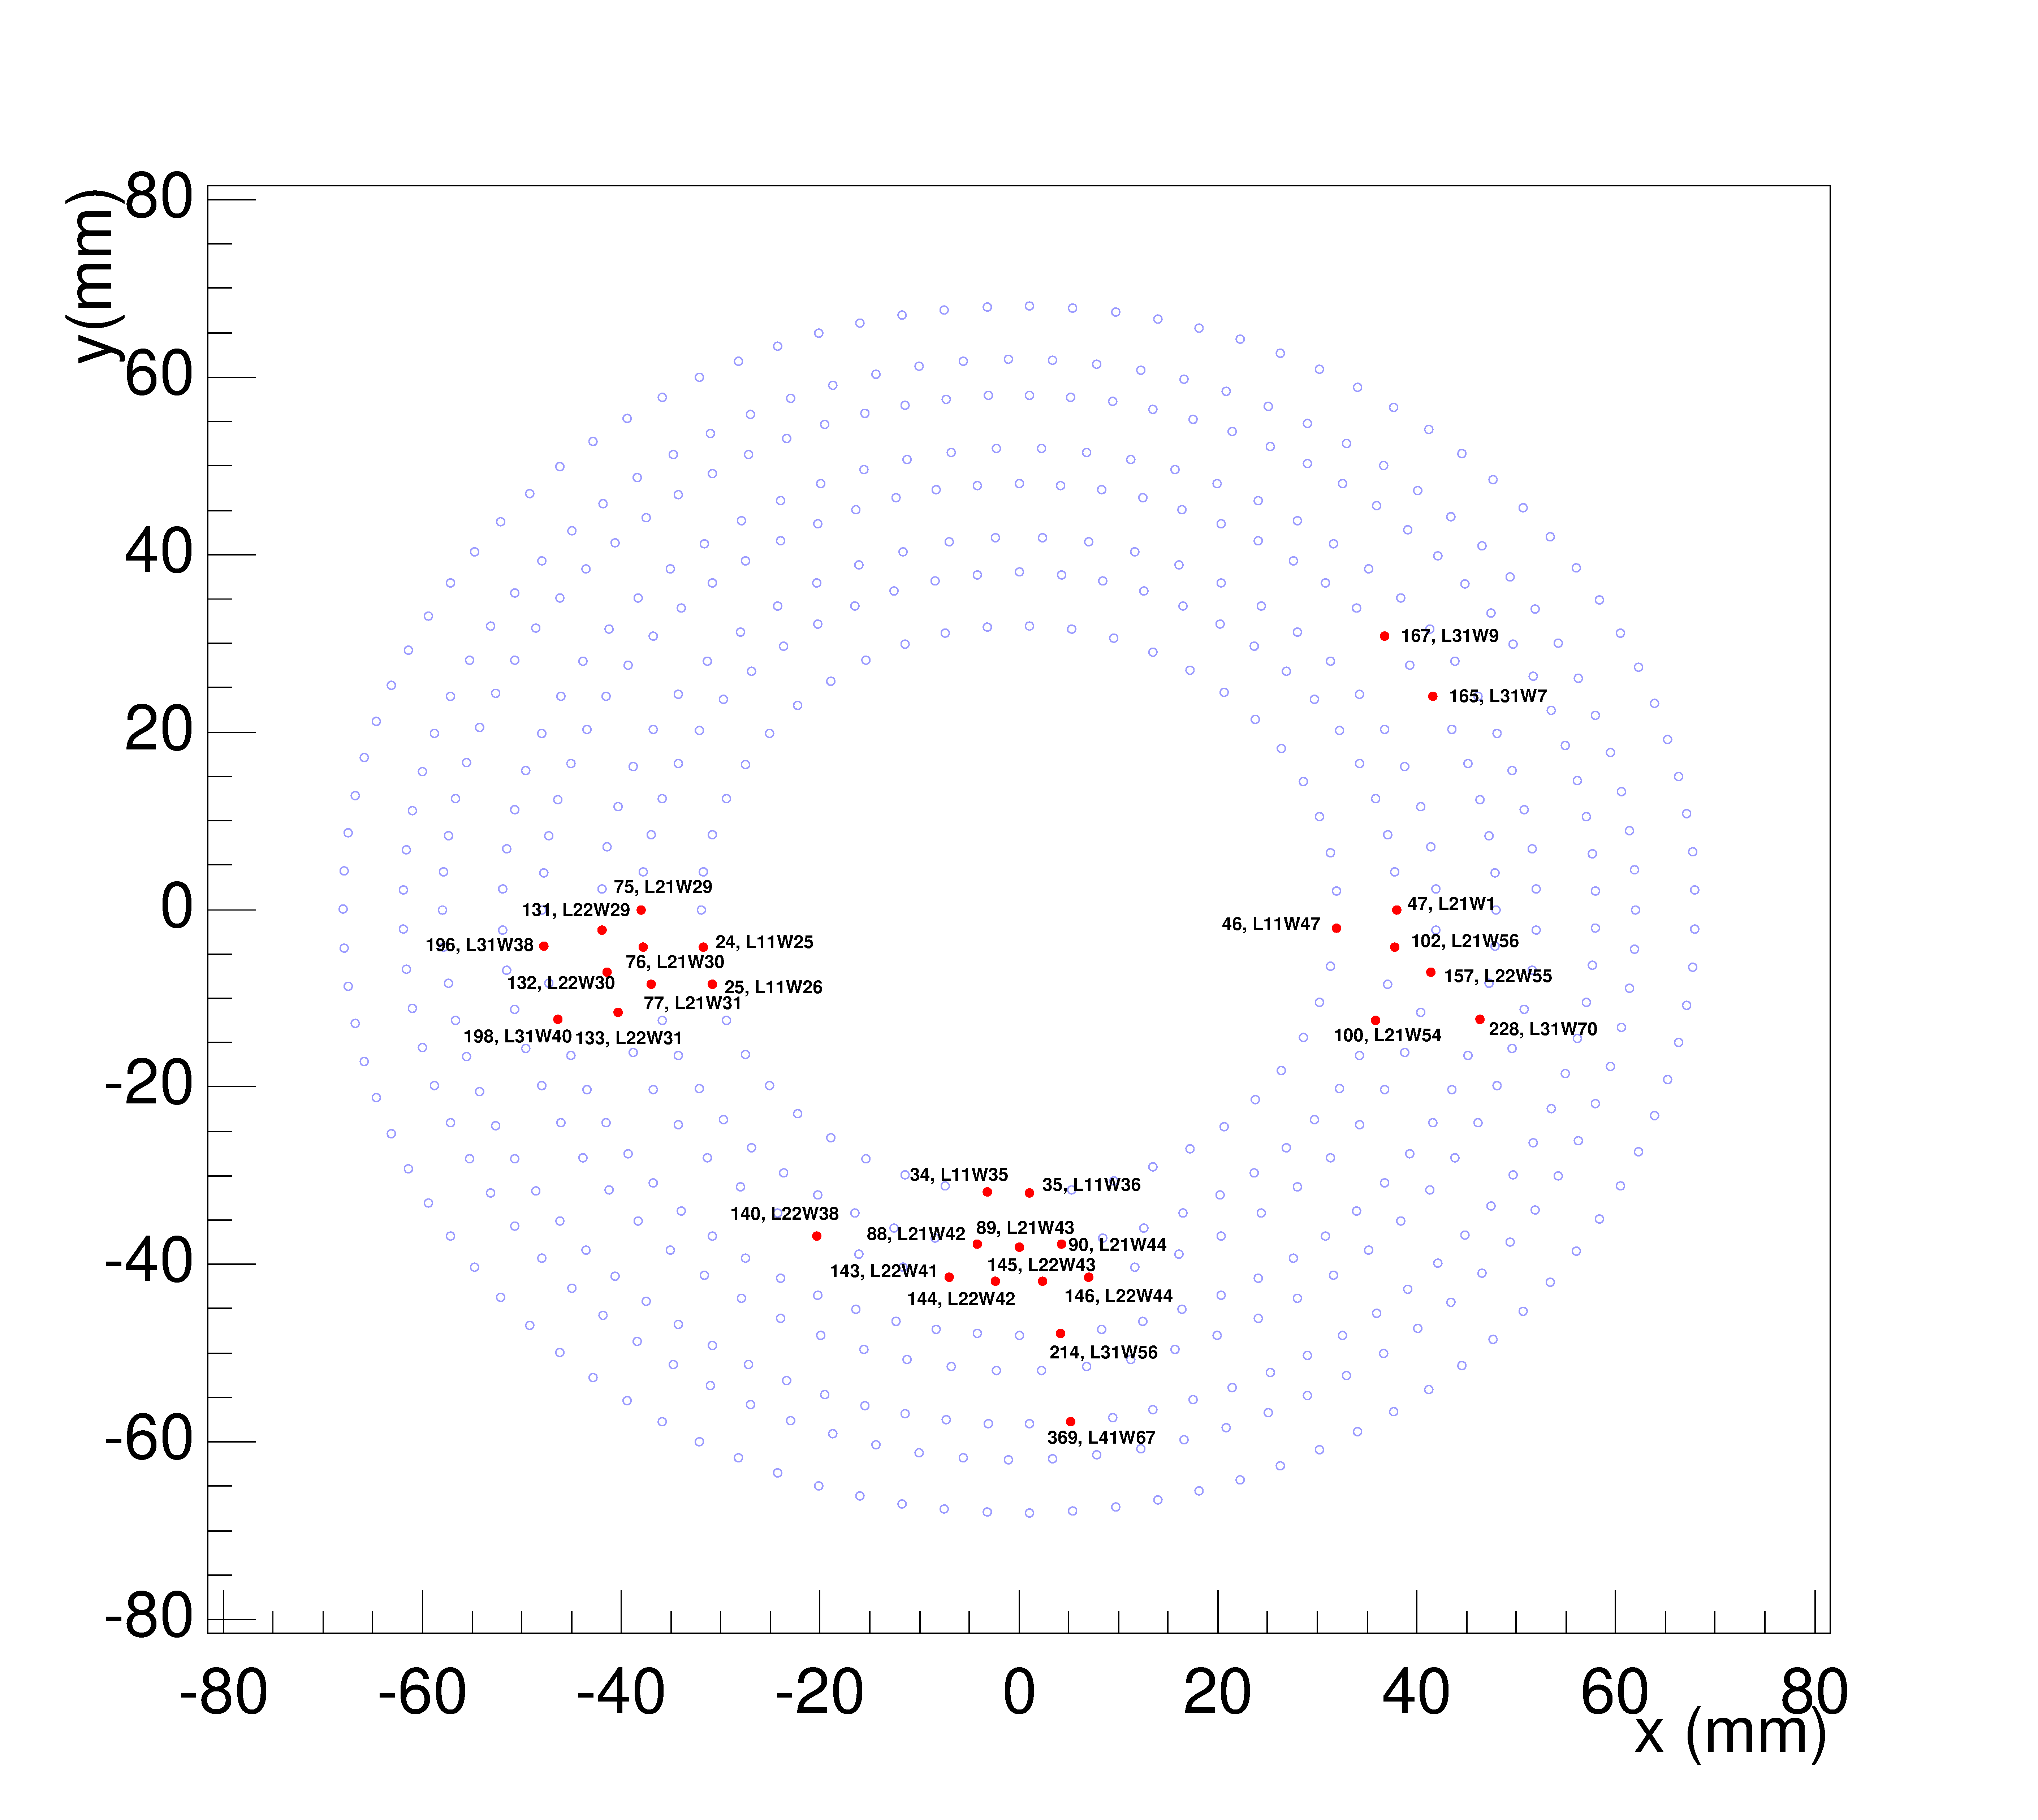
\includegraphics[width=0.48\textwidth]{figures/bad_wires_xy_view.pdf} &
        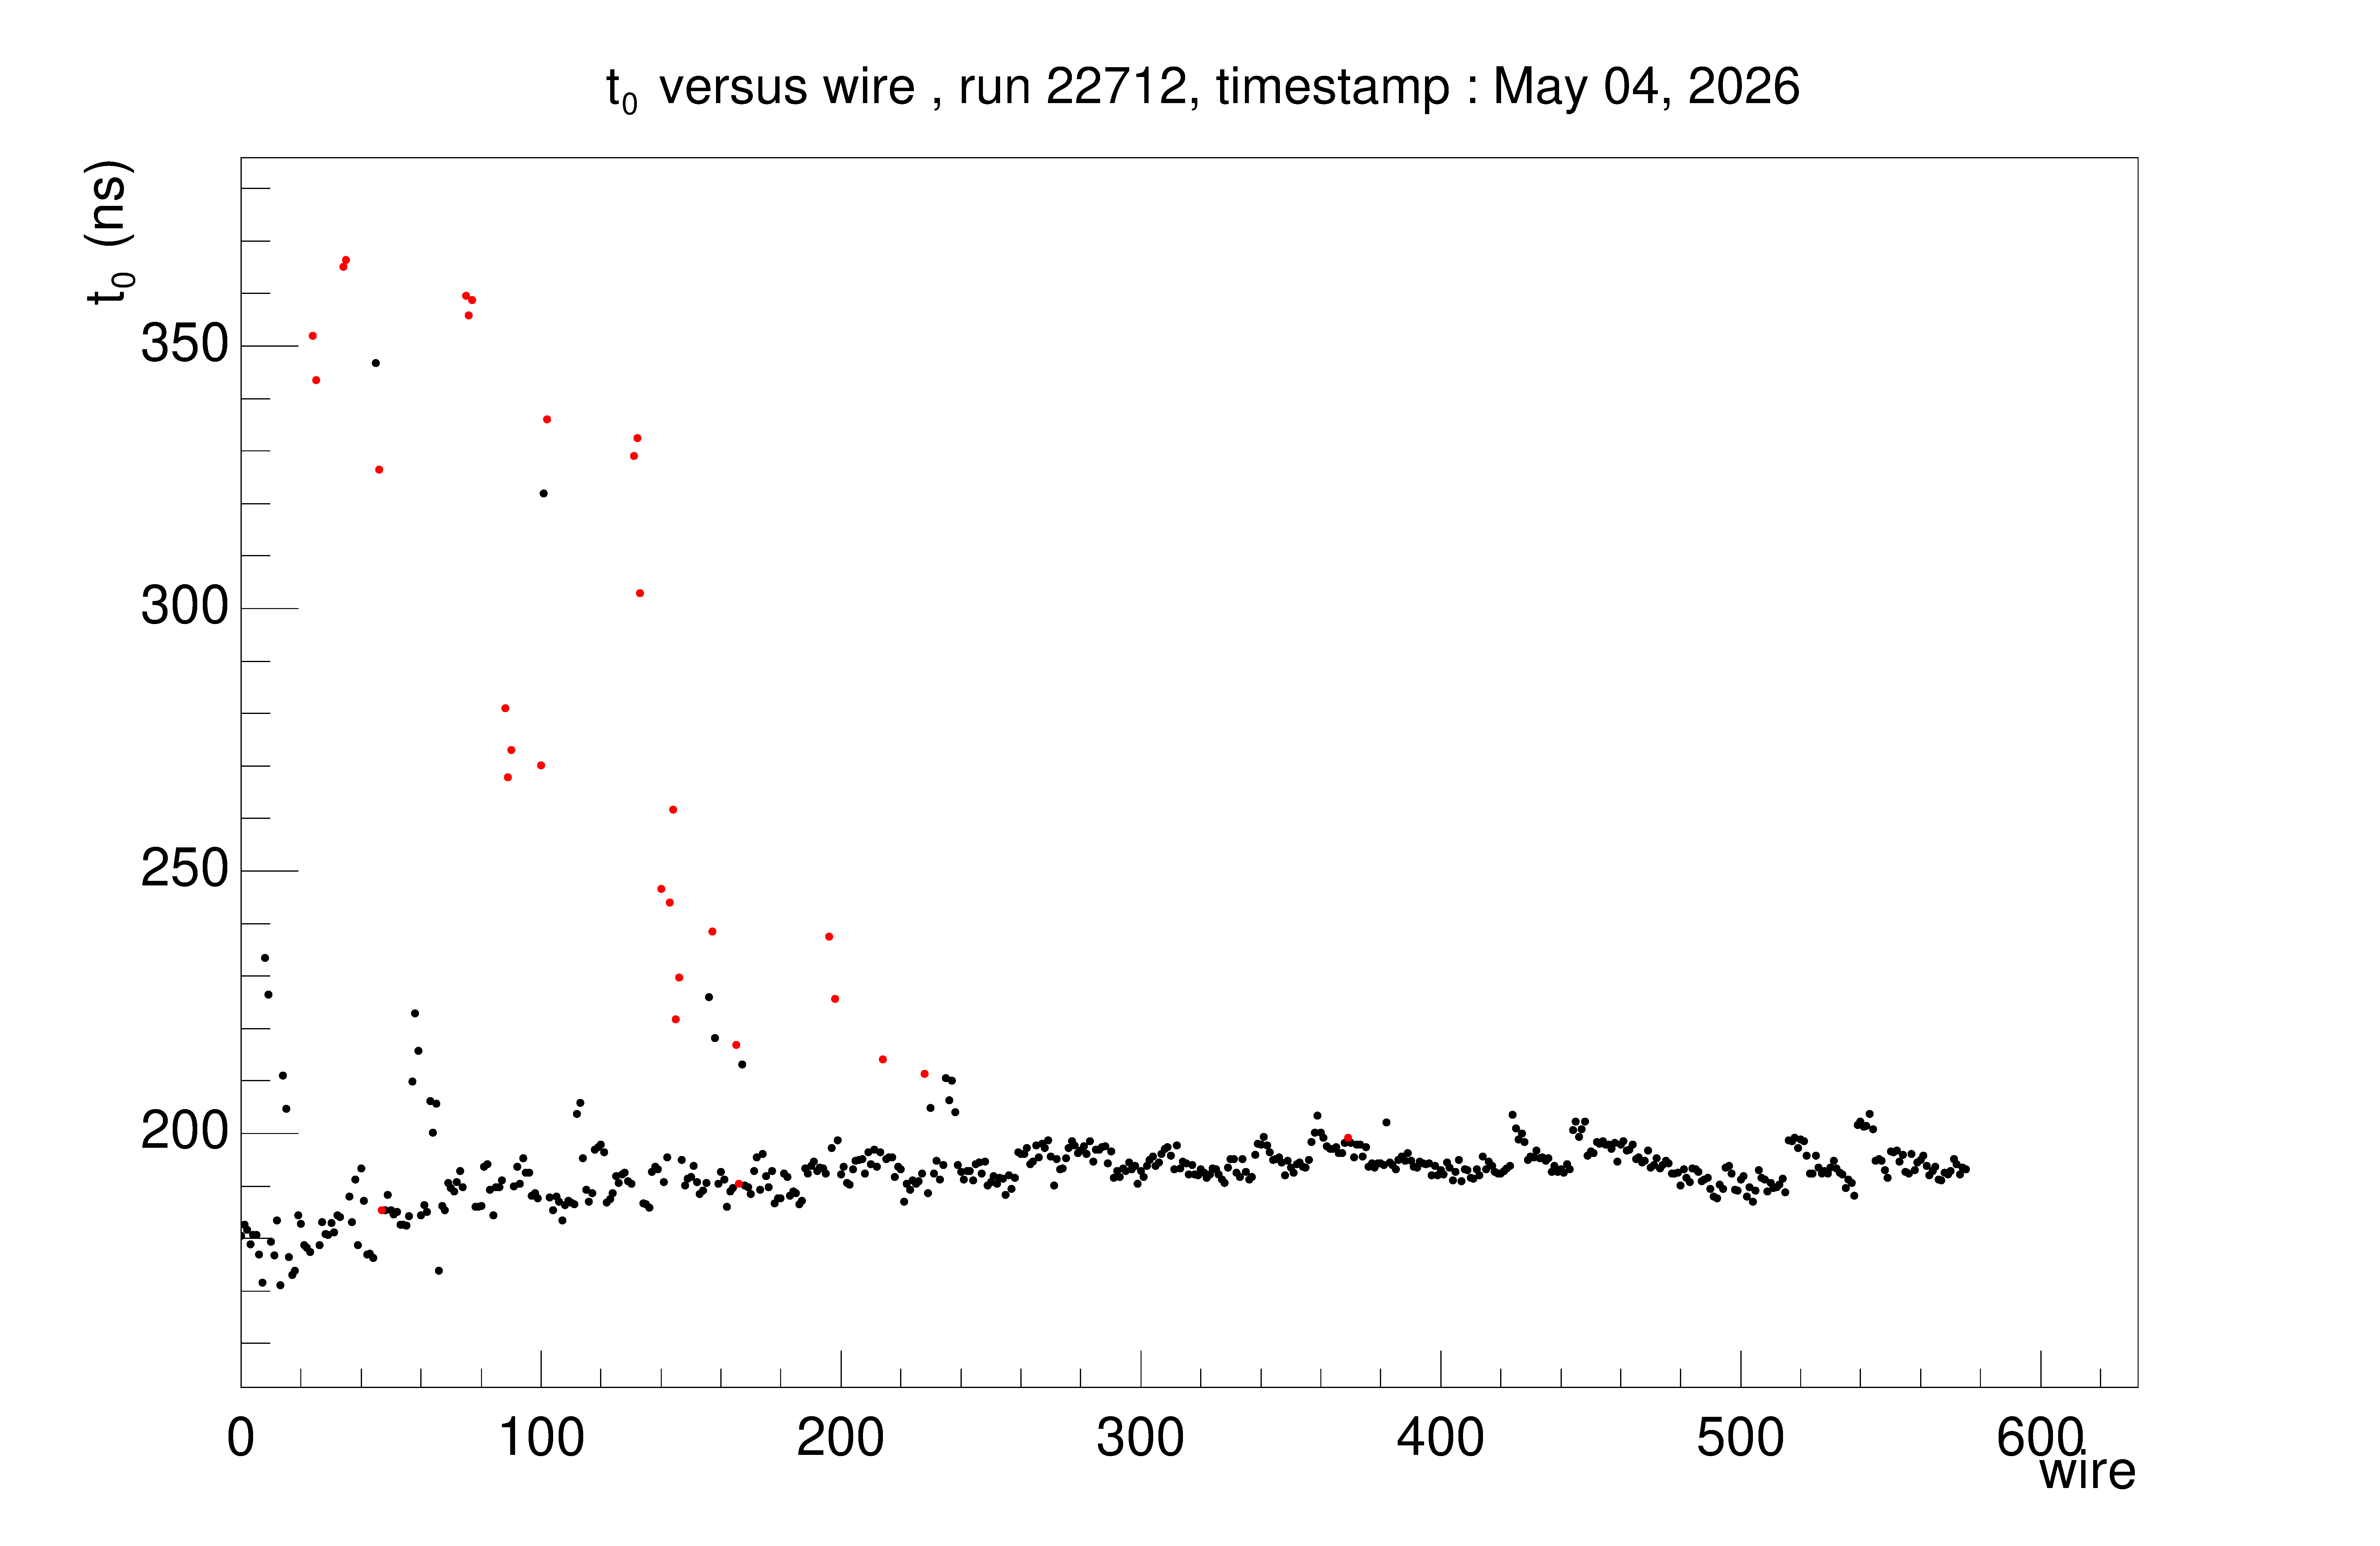
\includegraphics[width=0.48\textwidth]{figures/bad_wires_vs_t0.pdf}
    \end{tabular}

    
\end{frame}

\begin{frame}{Updates - wire swaps}
    \begin{itemize}
        \item Bad wires before (left) and after (right) $t_0$ correction
        \item As some distributions have been fixed, the number of possible swaps is reduced
        \item Examples:
    \end{itemize}

    \centering
    \vspace{0.2cm}

    \begin{tabular}{c|c}
        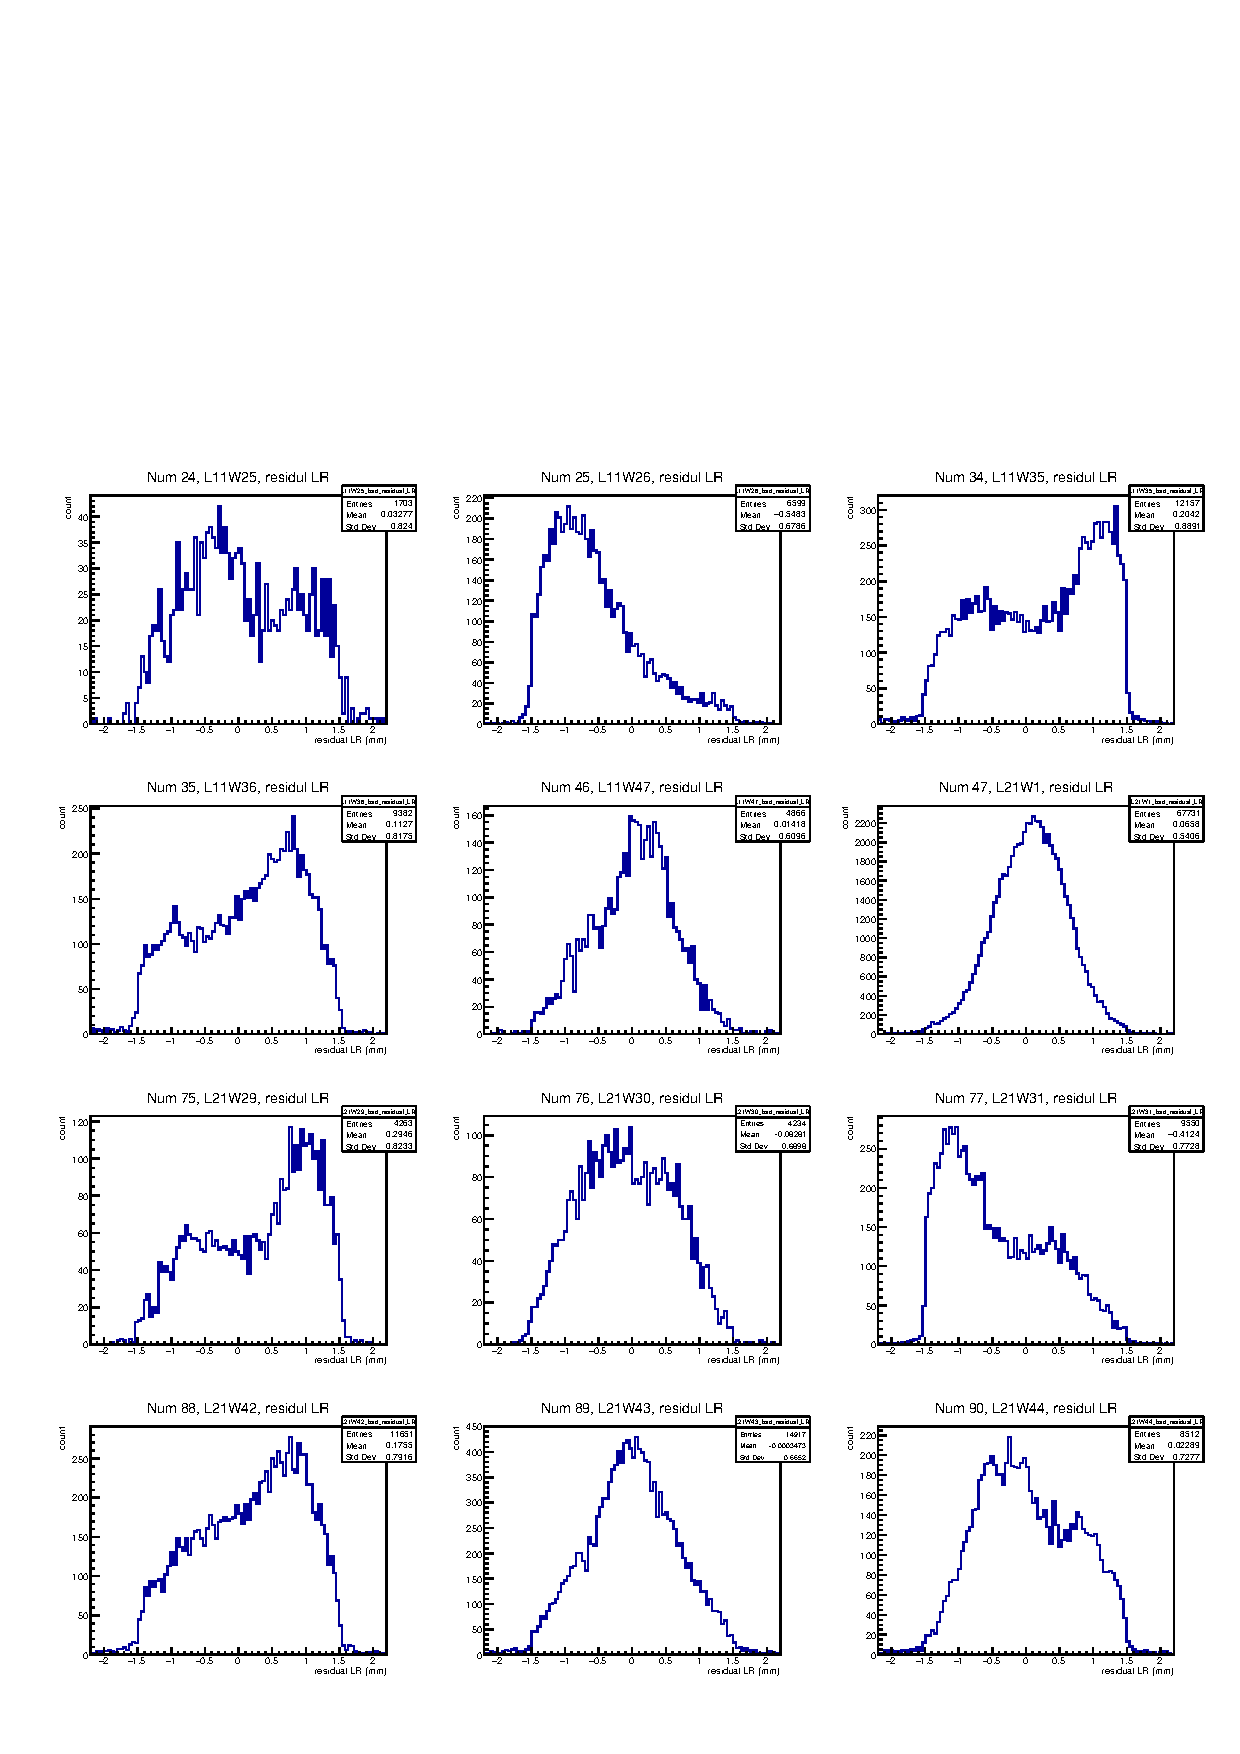
\includegraphics[width=0.48\textwidth,page=1]{figures/all_bad_wires_residual_LR_v2.pdf} &
        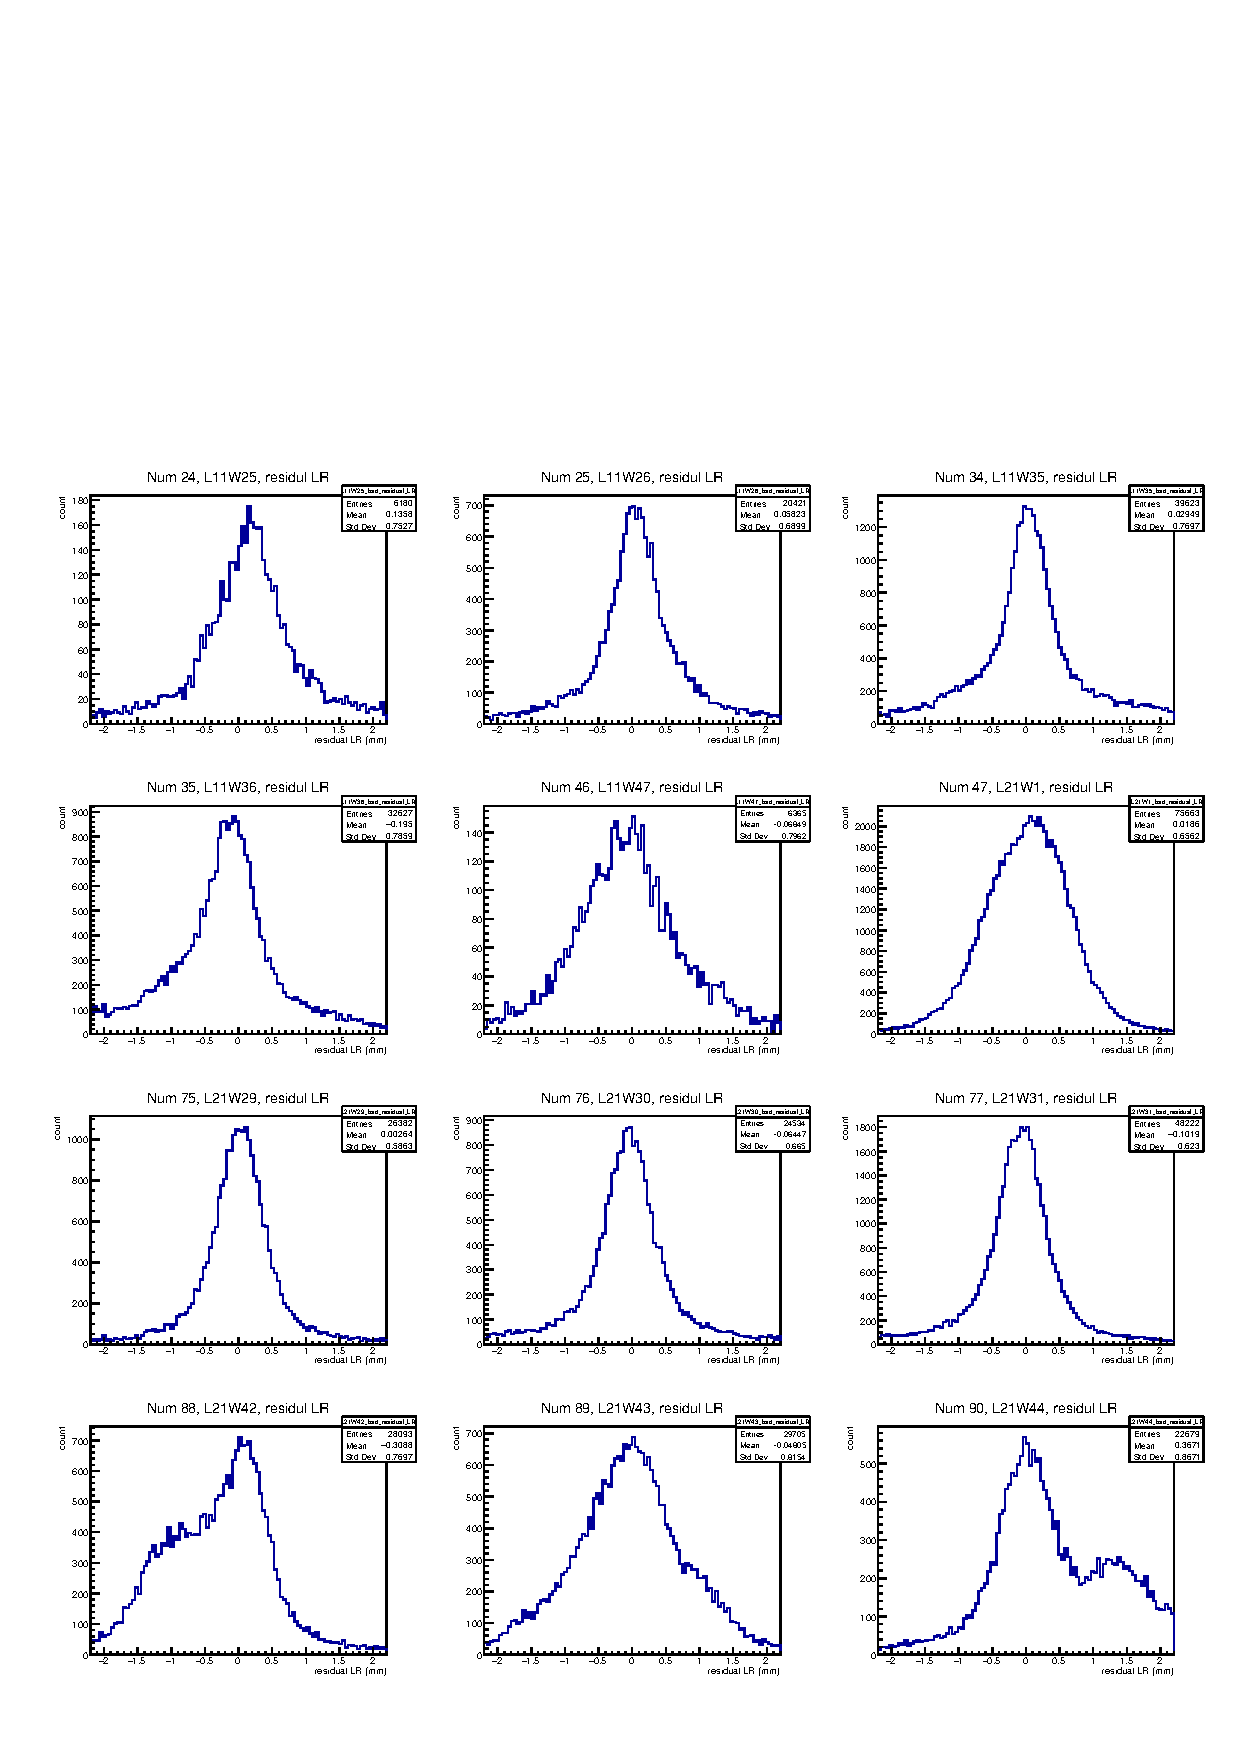
\includegraphics[width=0.48\textwidth,page=1]{figures/all_bad_wires_residual_LR_v13.pdf}
    \end{tabular}
    
\end{frame}


% \begin{frame}{Backup slides}
%     \begin{itemize}
%         \item Procedure:
%             \begin{enumerate}
%                 \item We looked at elastic events : electron + track (here: collection of hits only)
%                 \item We computed the theoretical momentum vector of the track $\vec{p}$
%                 \item We made the propagation without doing any fit (i.e no KF correction)
%                 \item We looked at {\color{blue} residual\_LR} (left-right) $\longrightarrow$ sensitive to the alignment
%             \end{enumerate}
%     \end{itemize}
    

%     \vspace{0.2cm}
%     \centering
%     \begin{minipage}{0.42\textwidth}
%         \includegraphics[width=\linewidth]{figures/build/illustration_residual_type.pdf}
%     \end{minipage}

% \end{frame}






\end{document}


